\documentclass[conference,10pt]{IEEEtran}
%\documentclass[conference,draft,onecolumn]{IEEEtran}
% useful packages, copy and paste from diff sources

\usepackage[english]{babel}
\usepackage[T1]{fontenc}
\usepackage{cite,url,color} % Citation numbers being automatically sorted and properly "compressed/ranged".
\usepackage{graphics,amsfonts}
\usepackage{epstopdf}
\usepackage[pdftex]{graphicx}
\usepackage[cmex10]{amsmath}
%\DeclareMathOperator*{\argmax}{arg\,max}
%\DeclareMathOperator*{\argmin}{arg\,min}
% Also, note that the amsmath package sets \interdisplaylinepenalty to 10000
% thus preventing page breaks from occurring within multiline equations. Use:
\interdisplaylinepenalty=2500
% after loading amsmath to restore such page breaks as IEEEtran.cls normally does.
\usepackage[utf8]{inputenc}
% Useful for displaying quotations
%\usepackage{csquotes}
% Compact lists
%\let\labelindent\relax
\usepackage{enumitem}

%tikz figures
\usepackage{tikz}
\usetikzlibrary{automata,positioning,chains,shapes,arrows}
\usepackage{pgfplots}
\usetikzlibrary{plotmarks}
\newlength\fheight
\newlength\fwidth
\pgfplotsset{compat=newest}
\pgfplotsset{plot coordinates/math parser=false}

\usepackage{algorithm}
\usepackage{algorithmic}
%\usepackage{algpseudocode}

\usepackage{array}
% http://www.ctan.org/tex-archive/macros/latex/required/tools/
%\usepackage{mdwmath}
%\usepackage{mdwtab}
%mdwtab.sty	-- A complete ground-up rewrite of LaTeX's `tabular' and  `array' environments.  Has lots of advantages over
%		   the standard version, and over the version in `array.sty'.
% *** SUBFIGURE PACKAGES ***
%\usepackage[tight,footnotesize]{subfigure}
\usepackage{subfig}

\usepackage[top=1.5cm, bottom=2cm, right=1.6cm,left=1.6cm]{geometry}
\usepackage{indentfirst}

\usepackage{times}
% make sections titles smaller to save space
%\usepackage{sectsty}
%\sectionfont{\large}
% enable the use of 'compactitem', a smaller 'itemize'
%\usepackage{paralist}

% MP
% to split equations using dmath env
\usepackage{breqn}
% nice rules in tables
\usepackage{booktabs}

%\setlength\parindent{0pt}
\linespread{1}

% MC
\newcommand{\MC}[1]{\textit{\color{red}MC says: #1}}
\newcommand{\AZ}[1]{\textit{\color{blue}AZ says: #1}}
\newcommand{\MP}[1]{\textit{\color{green}MP says: #1}}

\usepackage{placeins}

%%%%%%%%%%%%%%%%%%%%%%%%%%%%%%%%%%%%%%%%%%
\begin{document}
%%%%%%%%%%%%%%%%%%%%%%%%%%%%%%%%%%%%%%%%%%
\title{Proactive	caching	in	high	speed	scenarios	with	mmWave	communications}

\author{\IEEEauthorblockN{Ludovico Frizziero,
				  		Alberto Suman,
			  	  		Anthony Dell'Eva}
\IEEEauthorblockA{Department of Information Engineering, University of Padova -- Via Gradenigo, 6/b, 35131 Padova, Italy\\Email: {\tt\{ludovico.frizziero,alberto.suman,anthony.delleva\}@studenti.unipd.it}
}}

\maketitle

%% enable page numbering %%
%\thispagestyle{plain}
%\pagestyle{plain}
%%%%%%%%%%%%%%%%%%%%%%%%%%%

\begin{abstract}
This is a template for a scientific research paper. The abstract is a super brief summary of what you do in the paper.
\end{abstract}

%%%%%%%%%%%%%%%%%%%%%%%%%%%%%%%%%%%%%%%%%
\section{Introduction}\label{sec:intro}
%%%%%%%%%%%%%%%%%%%%%%%%%%%%%%%%%%%%%%%%%
The introduction is structured as follows
\begin{itemize}
	\item What are we talking about: description of the addressed problem. 
\item Motivation: why the problem is important.
\item Novelty: how you contribute to advance the state of the art
\item Results: summary of the main findings 
\end{itemize}

%%%%%%%%%%%%%%%%%%%%%%%%%%%%%%%%%%%%%%%%%%%%
\section{Related Work}\label{sec:sota}
%%%%%%%%%%%%%%%%%%%%%%%%%%%%%%%%%%%%%%%%%%%%
The Related Work section contains an analysis of the most relevant related literature (remarking the shortcomings that are addressed in your work)

%%%%%%%%%%%%%%%%%%%%%%%%%%%%%%%%%%%%%%
\section{System Model}\label{sec:symo}
%%%%%%%%%%%%%%%%%%%%%%%%%%%%%%%%%%%%%%

\begin{figure*}
	\centering
	
\includegraphics[width=18cm, height=10cm]{placeholder.png}
	\caption{representation of the highway sector.}
	\label{fig:highway_sector}
\end{figure*}

This section describes the model used for the simulation. In particular we discuss about the highway scenario, the wireless network architecture and, finally, the proposed solution for the proactive caching problem.

\subsection{Highway Scenario}
In the simulation we utilize a 1 km straight sector of the highway with three lanes for each direction. The sector is represented in [Fig. \ref{fig:highway_sector}]. For every iteration we consider a single user entering the road in one of the lane which is randomically chosen. The user's expected speed is $v_0$, while the instanteneous speed varies every $dt = 0.1\, s$ such as
\begin{equation}
	\label{eq:speed}
	v = v_0+a\cdot dt \quad [m\!/\!s]
\end{equation}
where $a$ indicates the acceleration, which is chosen randomically each second between $a_{min}=-10\,m\!/\!s^2$ and $a_{max}=5\,m\!/\!s^2$. The speed the user can have is also bounded to be in the interval $v \in v_0 \pm v_0 \cdot 10\%$. This is a somewhat hard constraint, although not completely unrealistic.

\subsection{Network Architecture}
For this paper we used a 5G wireless network architecture to provide high data rate in most coverage areas. The parameters of the channel are given in the table. Base stations (BS) are deployed in each side of the road according to a Poisson distribution with mean $\lambda_{BS}$, hence the total expected amount of base station per sector is $2\lambda_{BS}$. The distance from a BS to the next one within the same row is given as
\begin{equation}
	\label{eq:distance}
	\delta_{i, j} = \frac{1000}{\lambda_{BS}}+u \quad [m]
\end{equation}
where $u$ is generated by an uniform distibution in the interval $[-500\cdot\lambda_{BS}^{-1},500\cdot\lambda_{BS}^{-1}]$. This means that usually BSs tend to be uniformly spaced apart, but it can happen that some BS may end up being very close one another.  

\begin{table}
	\caption{Parameters of the channel}
	\label{tab:params}
	
\end{table}

The number of users for each BS is renewed every second with a value given by a poisson distribution with parameter $\lambda_{U\!E}$. Thus the available bandwidth for the user at the i-th BS is
\begin{equation}
	\label{bandwidth}
	BW_{U\!E,i} = \frac{BW}{m_i}
\end{equation}
where $m_i$ indicates the number of users at the i-th BS.
Every $dt$ the rate from the i-th BS to the user equipment (UE) is calculated as
\begin{equation}
	\label{eq:rate}
	r_i = BW_{U\!E,i}\cdot\log_2(1+SINR) \	
\end{equation}
where in the SINR computation we used the path-loss model given by
\begin{equation}
	(PL_i)_{dB} = 32.4+20\log_{10}(d)_m+20\log_{10}(f_c)_{M\!H\!z}+\Psi
\end{equation}
with $\Psi\sim \mathcal{N}(0,6)$ taking into account the shadowing. We consider also an outage threshold, below which it is set $r = 0$.

Furthermore, the BSs and the UE are provided with electronically steerable directional antennas. BSs take advantage of MIMO techniques, as spatial multiplexing and spatial beamforming to improve, respectively, rate and channel gain. The latter is computed from the Channel State Information matrix, which is completely updated every $3\cdot dt$ seconds, while signal scattering due to subpaths is recomputed every $dt$.

Finally, the BSs' network drives the handover in an optimal way: the users is forced to connect only to those BS that have memory available for him, in an order induced by the UE's travel direction, and only when it is proper to due so, that is only when the UE is about to enter the support region of the next BS. The concept of support region is introduced later in [eq. \ref{eq:support-region}].

\subsection{User Behavior}

The user needs to download a huge file $F$ (such that it can't be downloaded entirely within the premises of the highway sector we consider) from the internet. We consider the file to be compressed, such that to require a minimum rate $\mu_{U\!E} \in [0.06, 0.15]$ Gbits/s in order to be played back/consumed correctly by the user. The user also has at its disposal a buffer $\Omega$ that allows to store 15 seconds of content, that is
\begin{equation}
\Omega = 15 \cdot \mu_{U\!E} \quad [bits]
\end{equation}

 As soon as the UE is connected to a BS that has memory allocated for him, it starts downloading the available chunk of file with the rate $r_i$ provided by the connection, and to store it in its buffer. There is no flow control, therefore it may happen some portion of the file are lost due to buffer overflow. Lost data are not currently retransmitted. We also consider the download process as a stream of bits rather that packets, since channel errors are not considered. This allows to evaluate for maximum and ideal performances of our system.
 
\section{Proposed Solution}
 
This section describes the problem we want to solve, then it provides the solution, correlated with pseudocode for the solver for the related optimization problem.

\subsection{Problem Statement}

We want to achieve as uniform as possible performances of our system across all range of speeds the user can have, regardless of the underlying BS density and memory availability in each of them, while keeping the communication overhead among the central controller (CC), required for coordination, and all the BSs as low as possible. 

The overhead is reduced thanks to two main assumption: each highway sector is thought as independent from the others, and therefore each of them has it's own local controller; every BS manages it's memory regardless of the others. When a UE is going to enter the sector, the relative CC is notified. It then computes an optimal size of memory to allocate to the eventually selected BS based on the actual mean speed of the UE and the density of base stations on the sector, as
\begin{equation}
m = \alpha_{v_0, \lambda_{B\!S}} \cdot \tau \cdot \mu_{U\!E} \quad [bits]
\end{equation}

where $\tau = (1000/\lambda_{B\!S})/v_0$ is the mean connection time to a BS the UE can experience on the sector, and $\alpha_{v_0, \lambda_{B\!S}} > 0$ is a scale factor used to tune performances. In particular it is strictly tied to the optimal number of base stations the CC ends up allocating along the highway. Every BS within the premises of the CC must then only report if it has such memory space available or not. This eases communication overhead because the CC doesn't have to keep a record of the memory state for each base station constantly updated.

Now that the CC knows all the candidate BSs, an optimal number among them must be chosen to receive a chunk of the file requested by the UE. This is possible by defining the concept of support of the i-th BS as
\begin{equation}
\label{eq:support-region}
S_i = g_i(m)\frac{v_0}{\mu_{U\!E}} \quad [m]
\end{equation}

that is, for how many meters the UE can travel only relying on its buffer after he downloaded all the memory $g_i(m)$ the i-th BS had allocated for him, before experiencing file playback freezing. This measure, due to $v_0$, is of course, only in expectation. The support is also thought as centered on its relative BS, but this is not important as long as its starting point is decided with a common rule for each BS. Instead, $g(\mathbf{m})|_i \doteq g_i(m)$, where $\mathbf{m} \in \{0, m\}^N$ is the vector containing the memory report for each BS in the sector, is a function introduced later, that determines how much memory the CC eventually allocates to the i-th BS. The optimal number of BSs to choose is then found as $\mathbf{S}^T\mathbf{x} \approx 1000$, where $\mathbf{x} \in \{0,1\}^N$ is the (binary) choice vector outputted by the CC, and  $\mathbf{S} \in \mathbb{R}_+^N$ is the vector that contains the support for each BS.

Finally, it is also necessary to evenly distribute the chosen BSs along the sector, to assure buffer overflows are minimized and playback freezing is avoided. To this avail the final optimization problem has a cost term that depends on a vector $\mathbf{d} \in \mathbb{R}_+^N$ which captures the relevant distances among chosen base stations, that is, given $\mathbf{x} \in \{0,1\}^N$, each component is defined as

\begin{figure}[t]
	\centering
	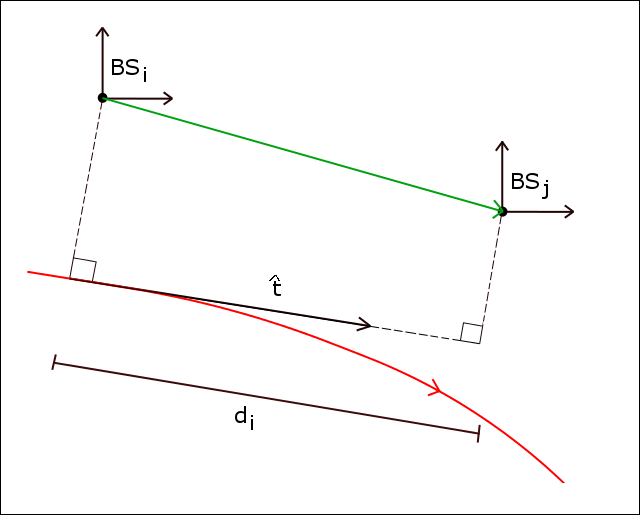
\includegraphics[width=9cm]{BS_distance.png}
	\caption{representation of minimum distances from [eq. \ref{eq:dists}] }
	\label{fig:min_dists}
\end{figure}

\begin{equation}
\label{eq:dists}
d_i = \min_{j \textrm{ s.t. }x_j = 1} |<pos_w(BS_i) - pos_w(BS_j), \hat{t}_{w, i}>|
\end{equation} 

Here $\hat{t}_{w, i}$ is the unitary norm tangent to the travel direction (predicted along the sector) of the UE in world coordinates, evaluated on the perpendicular of the i-th BS, while $pos_w(BS_i)$ is the position of the i-th BS in world coordinates. A representation is visible in [Fig.\ref{fig:min_dists}].

\subsection{Optimization Problem}

The proposed optimization problem therefore is

\begin{center}
	\begin{tabular}[h]{|c|}
		
		\hline
		OPTIMIZATION PROBLEM \\
		\hline
		\makebox[8.6cm]{
			$			
			\begin{array}{l l l l l l}
				\null \\
				\mathbf{x} \in \underset{\mathbf{x} \in \{0,1\}^N}{argmax} {\textrm{ } \sum_i{g_i(m)x_ie^{-\frac{(\mathbf{S}^T\mathbf{x} - 1000)^2}{2}}} - \lambda\left(\frac{\mathbf{d}^T\mathbf{x}}{2} - 1000\right)^2} \\[3ex]
				\textrm{such that:}\\[0.5ex]	
				\sum_i{g_i(m)x_i} \le F\\[0.5ex]		
				0  < g_i(m) \le min(m, \Omega) \textrm{ } \forall i \textrm{ s.t. } x_i  = 1 \textrm{,   0 otherwise}
				\null \\[2ex]
			\end{array}
			$
		}\\
		\hline
	\end{tabular}
\end{center}

where $\lambda > 0$ is a tradeoff parameter between memory allocation and its even distribution along the sector. The function $g(\cdot)$ allows for some flexibility from the CC side in distributing the memory, such that in some BS it may end up being less than what originally requested if needed for any reason. This is especially useful to avoid having overlapping supports between chosen base stations, because this may cause buffer overflow at the user side. In particular a useful expression for $g(\cdot)$ that minimizes such overlaps, given the almost uniform BSs' deployment assumed in this paper, is 

\begin{equation}
g_i(m) = min\left(\frac{1000\mu_{U\!E}}{v_0 ||\mathbf{x}||_0}, m\right)
\end{equation} 

because this makes the support $S_i$ become exactly the expected distance among BSs after having observed which one has been chosen, that is

\begin{equation}
S_i = \mathbb{E}{[\delta_{i, j}| \mathbf{x}]} =  \frac{1000}{\textrm{ }||\mathbf{x}||_0}
\end{equation} 

The expression $||\cdot||_0$ is the zero norm of a binary vector. The discussion made so far presents the solution that best maximizes our optimization problem given the geometric assumption it relies on. It is nonetheless possible to lessen the uniform constraint over $m$, or over $g(\cdot)$, but the solution becomes suboptimal. 

Finally we provide the pseudocode that solves the optimization problem in [Alg. \ref{alg:solver}], that runs approximately in $O(N^4)$ due to the update on $\mathbf{d}$. At first it solves the optimization problem by considering the requested amount $m$ for each BS. This way an optimal number of stations is selected, then it applies $g(\cdot)$ in order to minimizes support regions overlapping, while also maximizing the exponential to 1 as a (desired) byproduct.

\begin{algorithm}
	\caption{pseudocode to solve the optimization problem}
	\label{alg:solver}
	\begin{algorithmic}
		\STATE \textbf{Input:} $\mathbf{m} \in \{0, m\}^N, \textrm{ } F$, positions of each BS with respect to the world
		\STATE \textbf{Output:} $\mathbf{x} \in \{0, 1\}^N, \textrm{ } g(\mathbf{m}) \in \{0, g_i(m)\}^N$
		\STATE \null
			\STATE $\mathbf{x} \leftarrow \mathbf{0}$, $x_i \leftarrow 1$ for a random $i$
			\STATE $\mathbf{S} \leftarrow (\mathbf{m}v_0)/\mu_{U\!E}$
			\WHILE {$\mathbf{S}^T\mathbf{x} < 1000$ \OR $\mathbf{m}^T\mathbf{x} \le F$ }
				\STATE best_i $\leftarrow$ invalid index, best_k $\leftarrow -\infty$ 
				\FOR{$j \in \{1..N\}/\{i : x_i = 1\}$}
					\STATE $\mathbf{y} \leftarrow \mathbf{x}$, $y_j \leftarrow 1$
					\STATE $\mathbf{d} \leftarrow$ update distances as in [eq. \ref{eq:dists}] with reference to    	$\mathbf{y}$
					\STATE $k \leftarrow \mathbf{m}^T\mathbf{y} - \lambda\left(\frac{\mathbf{d}^T\mathbf{y}}{2} - 1000\right)^2$
					\IF{k > best_k}
						\STATE best_k $\leftarrow k$, best_i  $\leftarrow j$
					\ENDIF
				\ENDFOR 
				
				\IF{best_i \NOT invalid}
					\STATE $x_{best\_i} \leftarrow 1$
				\ELSE
					\STATE CONSTRAINTS NOT MET
				\ENDIF
			\ENDWHILE
			\STATE $g(\mathbf{m}) \leftarrow \mathbf{0}$
			\FORALL {i = \{1...N\}}
				\STATE 	$g_i(m)\leftarrow \frac{1000\mu_{U\!E}}{v_0||\mathbf{x}||_0}$ if $x_i=1$, 0 otherwise
 			\ENDFOR
			\RETURN $\mathbf{x}$, $g(\mathbf{m})$
	\end{algorithmic}
\end{algorithm}



%%%%%%%%%%%%%%%%%%%%%%%%%%%%%%%%%%%%%%%%%%%%%%%
\section{Results}\label{sec:res}
%%%%%%%%%%%%%%%%%%%%%%%%%%%%%%%%%%%%%%%%%%%%%%%

blablablablablablabla


\begin{figure*}[t]
	\label{fig:7BS_all_stats}
	\centering
	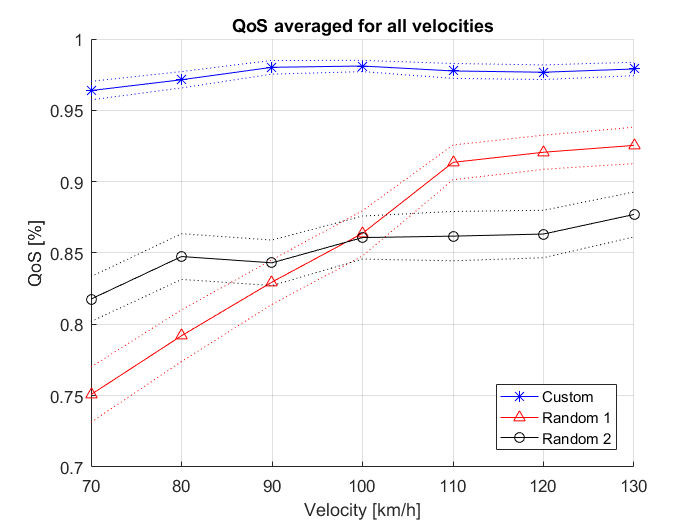
\includegraphics[width=9cm]{QoS.png} 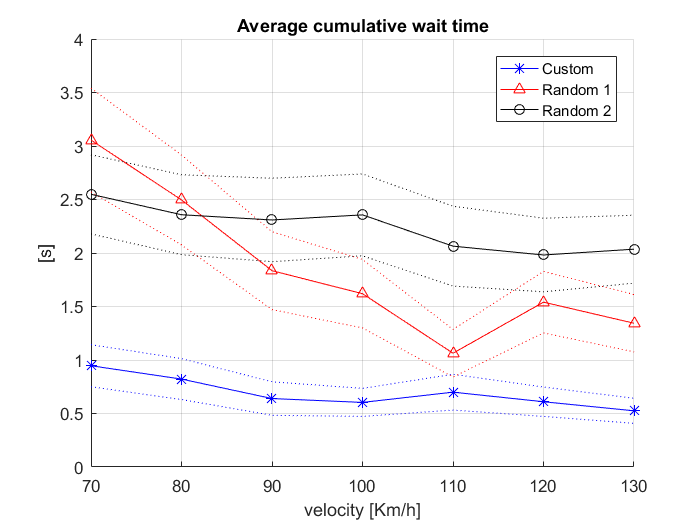
\includegraphics[width=9cm]{UE_wait_time.png}
	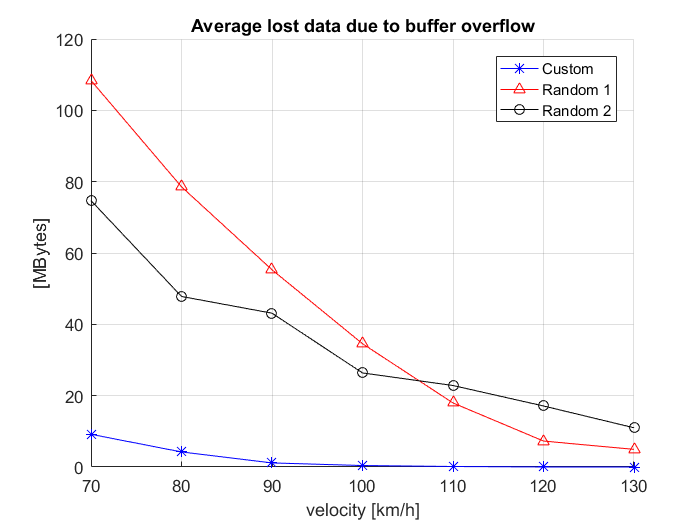
\includegraphics[width=9cm]{UE_buffer_overflow.png} 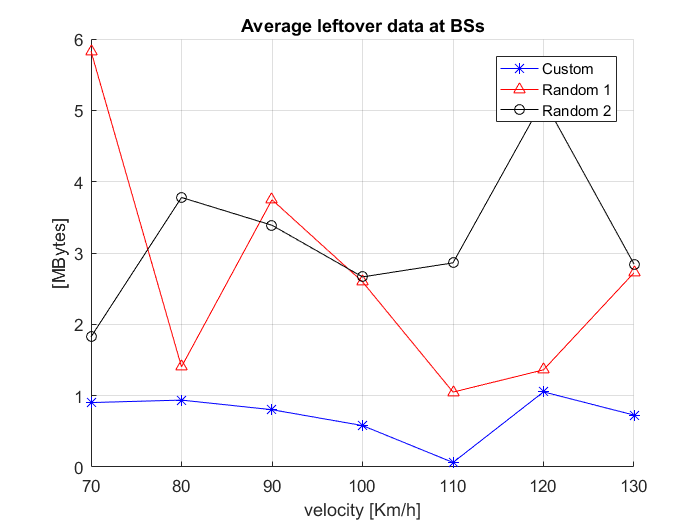
\includegraphics[width=9cm]{BS_leftover_data.png}
	\caption{Statistics for a sector with density of 14 BS. Confidence Intervals at 0.05\% are shown were relevant.}
\end{figure*}

\begin{figure}[b]
	\label{fig:7BS_buffer_load}
	\centering
	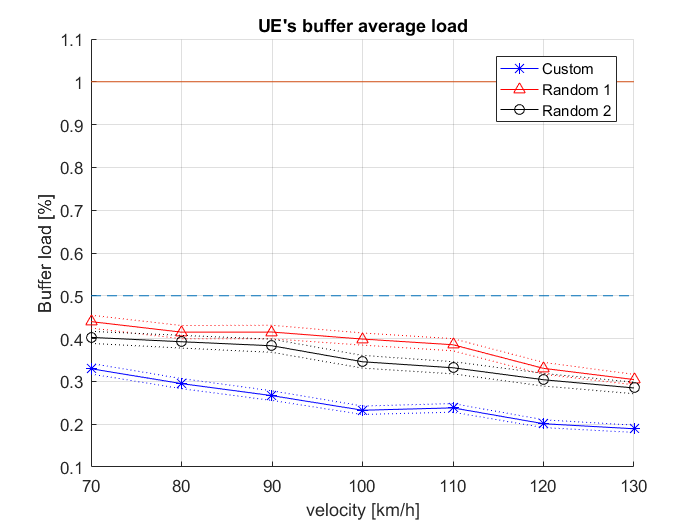
\includegraphics[width=9cm]{UE_buffer.png}
	\caption{Buffer load at UE side, for 14 BS per sector. Confidence intervals are at 0.05\%.}
\end{figure}

\begin{figure}[b]
	\label{fig:QoS_all}
	\centering
	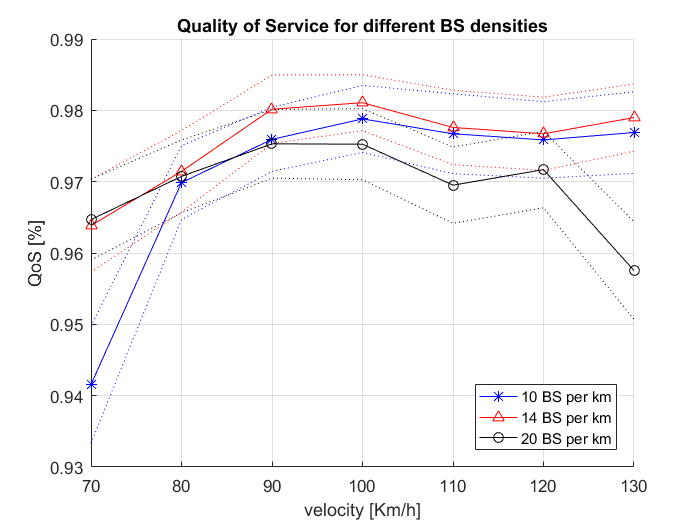
\includegraphics[width=9cm]{QoS_10-14-20-BS_densities.png}
	\caption{QoS for densities of 10, 14 and 20 BS per sector. Confidence intervals are at 0.05\%.}
\end{figure}

\begin{figure*}
	\label{fig:QoS_20km}
	\centering
	
\includegraphics[width=12cm]{placeholder.png}
	\caption{QoS for 20km long journey, 14 BS per sector. Confidence intervals are at 0.05\%.}
\end{figure*}

%%%%%%%%%%%%%%%%%%%%%%%%%%%%%%%%%%%
\section{Conclusions}\label{sec:conclusion}
%%%%%%%%%%%%%%%%%%%%%%%%%%%%%%%%%%%
Conclusions are a superbrief summary of what has been done and highlighting of the "take home message"

\end{document}
